\documentclass[pagenumber=off]{article}

\usepackage[pdftex]{graphicx}
\usepackage{xcolor}
\usepackage[a4paper,margin=0.7in,portrait]{geometry}
\usepackage{etoolbox}
\usepackage{hyperref}

%----------------------------------------------------------
\definecolor{coolblack}{rgb}{0.0, 0.18, 0.39}
%\AtBeginDocument{\color{coolblack}}
%----------------------------------------------------------

%%----------------------------------
\begin{document}

%%--- Title ---
\begin{titlepage}
\begin{center}
\vspace{1cm}
{\textcolor{gray}\today}\\
{\textcolor{gray}{\bf Udacity Nanodegree: Deep Reinforcement Learning }}\\
\vspace{1.5cm}
{\textcolor{coolblack}{\huge \bf III Project: Collaboration and Competition}}\\
\vspace{0.5cm}
{\textcolor{coolblack}{\Large \bf  Teaching two agents to play tennis via Multi Agent Reinforcement Learning}}
\par
\vspace{0.5cm}
%{\textcolor{coolblack}{\Large\itshape Solved using Deep Deterministic Policy Gradient (DDPG).}}\par
\vspace{6cm}
\end{center}
\tableofcontents

\vspace{4cm}

\begin{center}
{Alberto M. Cozzini}\\
\end{center}
\end{titlepage}

%----------------------------------
\section{Task}
For this project, two tennis players have to learn to control rackets to bounce a ball over a net.\\
Agents control the rackets in a continuous space, moving them back and forth and jump. 
If an agent hits the ball over the net, it receives a reward of +0.1. If an agent lets a ball hit the ground or hits the ball out of bounds, it receives a reward of -0.01. Thus, the goal of each agent is to keep the ball in play.

The task is episodic and in order to solve the environment the agents must get an average score of at least 0.5 over 100 consecutive episodes. Here is an example of benchmark solution.
%----------------------------------
\begin{figure}[!h]
  \centerline{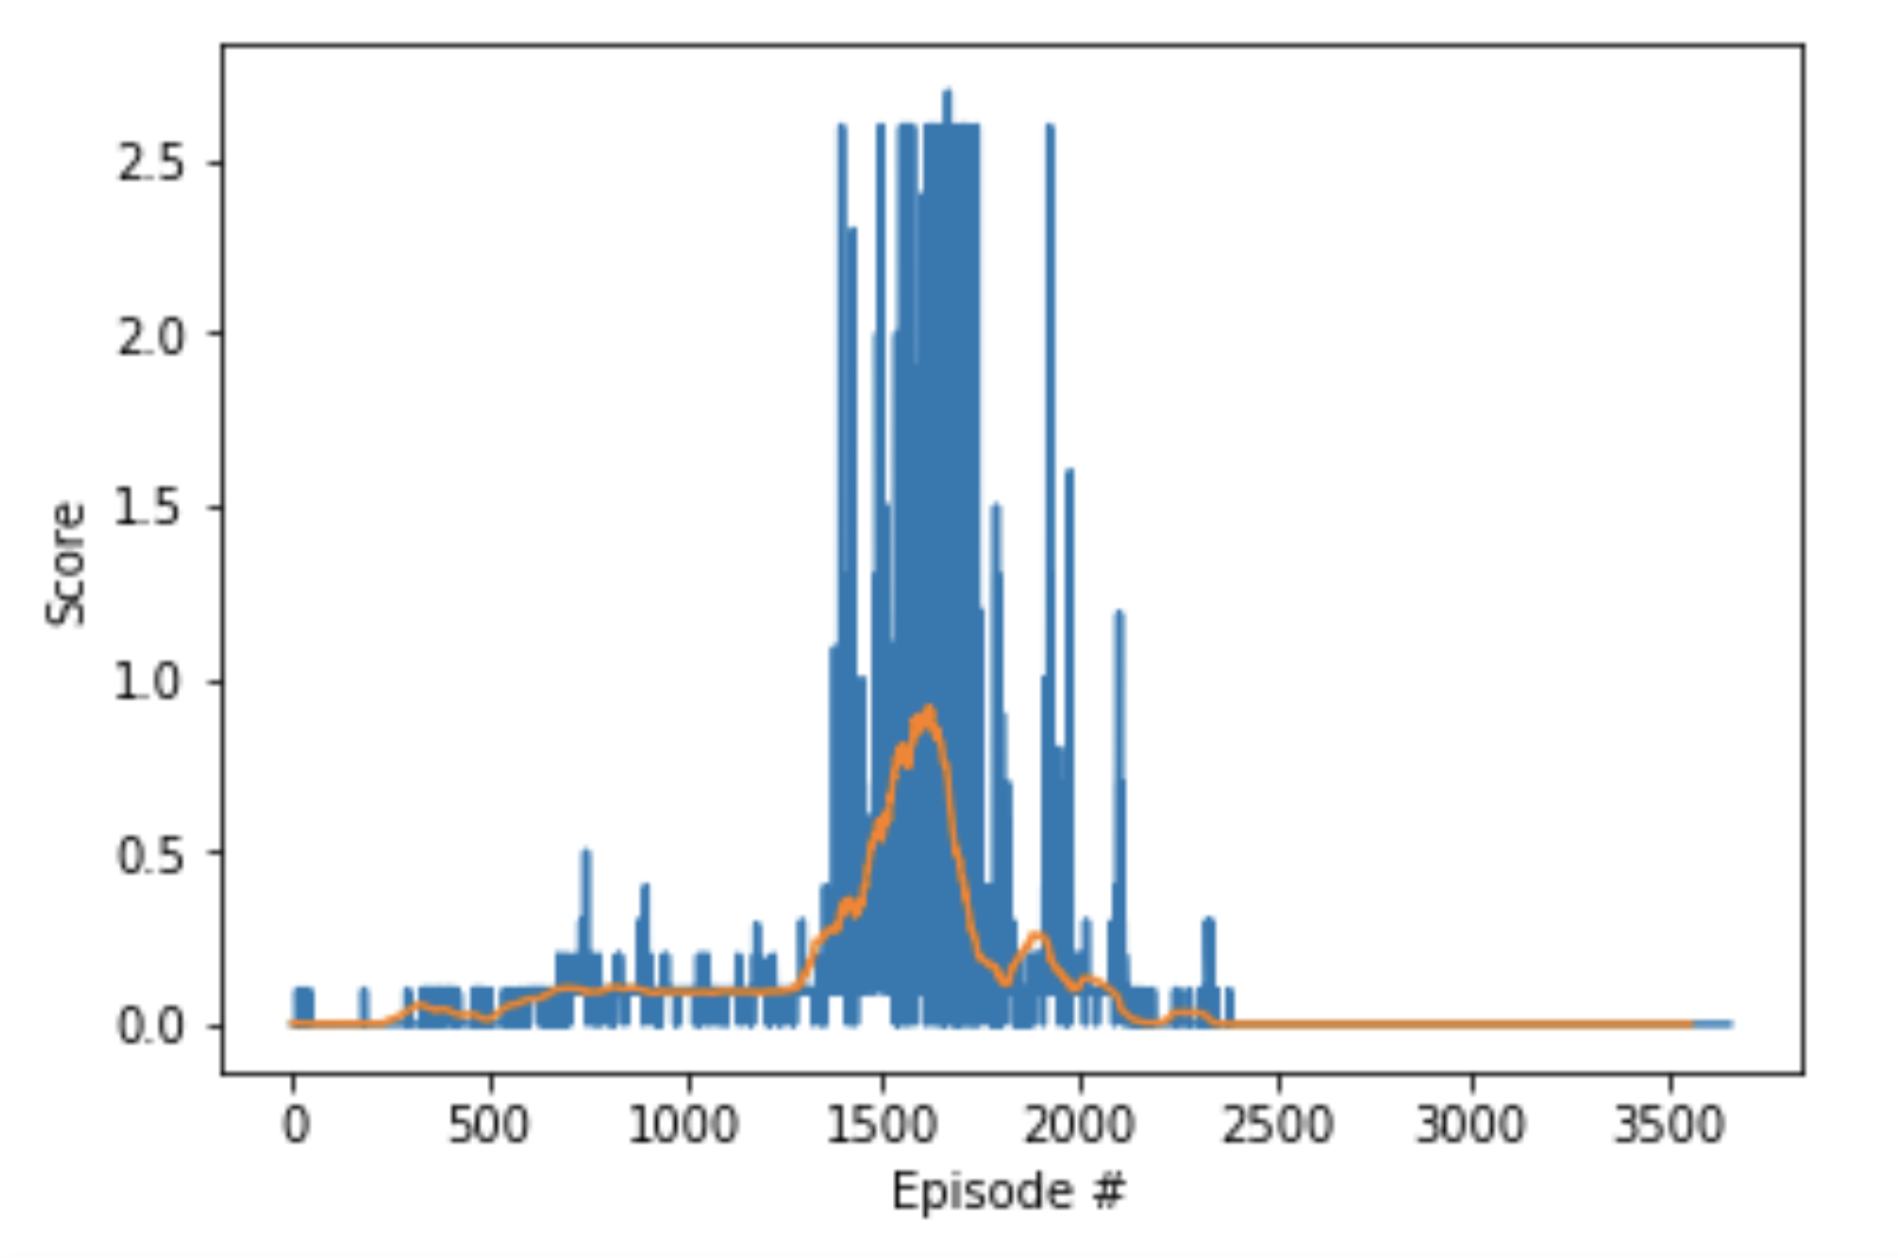
\includegraphics[page=1, height=6cm, width=12 cm, angle=0]{./Plots/Benchmark_Score.png}}
  \caption{Benchmark Implementation. It reaches an average score of at least 0.5 over 100 episodes.}
\end{figure}
%----------------------------------

%----------------------------------
\section{Tennis Environment}
The tennis environment is built on a Unity architecture.\\
The state space consists of 8 variables representing position and velocity of the ball. Each agent observe his own state space.
To catch the evolution of the game each agent observes at each step a stack sequence of 3 vectors of states space variables, i.e. 24 data points in total.
Given this information, the agent has to learn how to best select actions. Each action is a two dimensional vector, corresponding to the movement toward (or away from) the net, and jumping. Each scalar in the action vector should be a number bounded between -1 and 1.

\subsection{Discount Factor}
The utility function of the agent values the immediate reward more than the futures rewards which are discounted at a factor of 0.95 per time step.


\section{MADDPG Learning Algorithm}
We implement a Multi-Agent Deep Deterministic Policy Gradient (DDPG) as per the paper \href{https://arxiv.org/pdf/1706.02275}{Multi-Agent Actor-Critic for Mixed Cooperative-Competitive Environments}
It extends the single actor-critic DDPG agent from \href{https://arxiv.org/abs/1509.02971}{Continuous control with deep reinforcement learning} to a multi-agent framework.

As the DDPG framework, it is an off-policy actor-critic model free algorithm based on the deterministic policy gradient that can extended the advantaged of the standard deep Q-Learning to continuous action space.

The main advantage of this approach is that it still follows a decentralised execution where each agent is aware of only his own surroundings and follows his own policy. At the same time agents learn is more efficient via a centralised critic which observes other agents' state and actions.



\subsection{Loss Function}

As in Q-Learning, by the Bellman equation, the loss function for the critic network  of each agent is the mean square error between the expected Q values computed on the local network and the target Q values computed on the network with momentarily frozen weights.

The actor policy is updated using the sample policy gradient. We use the local policy network of each agent to find the optimal action given the state and then we feed it to our local Q-value function, which is what we want to maximise. 

\subsubsection{Optimiser}

The optimiser performs a stochastic gradient descent step on the loss function with respect to the network weights.\\
We implement the Adam optimisation algorithm with learning rate of 1e-3.\\


\subsubsection{Critic Gradient Clipping}

As suggested by the course notes, we tested the extra stabilising option of clipping the gradient when training the critic network to 1.


\subsubsection{Soft Update}

To improve stability of learning process and avoid oscillations, we keep separate local and target networks. While the two networks are identical clones, we only update the weights of the target network by interpolating old with new local weights by a factor of 1e-3.

\subsubsection{Periodic Update}

We tested without success the periodic update  


\subsection{Decaying Action Noise}
We need to add noise to our actions to force exploration. Nonetheless we want to force a decay of the noise with time.
The temporally correlated noise is generated via Ornstein-Uhlenbeck process with drift $\theta=0.15$ and volatility $\sigma=0.2$.
We initially scale the noise by a factor 2 that decays by 0.9999 after each episode.


\subsection{Experience Replay}
To make the learning process more stable and avoid aberration of the action-value Q function, we store and randomly replay some of the recent buffer of experiences, 1e6.
The number of experiences we store in hour memory is 1e6. Each time we sample uniformly at random a batch of 512 experiences.


%-------------------------------
\section{Model Architecture}

We have two separate neural networks to approximate non linear functions representing the actor policy function and the critic action-value function. 

\subsection{Actor Policy}
Each agent policy function takes in as input 3 consecutive arrays of 8 state observations.
We normalise the input before passing them to the neural network.
The neural network has two hidden layers. First layer has 256 fully connected nodes, the second has 128 nodes.
We use the leaky ReLU activation function which has the benefit of having a very small slope for $x < 0$.
The output is mapping to the 2 continuous actions with tangent activation function to bound each between -1 and +1.

\subsection{Critic}
The critic network approximates the Q-value function for a given state and action. In a Multi-Agent framework the critic has knowledge of all agents observations and actions.
Here too we first normalise the input observations array, 48 data points corresponding to the 24 states times 2 agents.
The first layer of the networks takes in only the state data points and maps them them to 256 nodes.
The second layer takes in the 256 plus the 4 actions from both agents. It has two fully connected hidden layers each of 128 nodes.
Again we use the Leaky ReLU activation function for each layer except for the output Q-value.


\newpage
%----------------------------------
\section{Solved}

It takes many episodes during which the agents more aggressively explore before they start to improve their performance and since then the progression is almost exponential.  

\begin{table}[h]
  \centering
    \begin{tabular}{|r|c|}
      \hline
      {\bf Episode} & {\bf Avg. Score} \\ 
      \hline
      1,000  & 0.009\\ 
      2,000  & 0.013\\
      3,000  & 0.06 \\
      4,000  & 0.10 \\
      5,000  & 0.11 \\
      6,000  & 0.12 \\
      7,000  & 0.12 \\
      8,000  & 0.21 \\
      {\bf 8,348}  & {\bf 0.50} \\
      9,000  & 0.64 \\
      10,000 & 0.92 \\
      \hline
    \end{tabular}
    \caption{Rolling average max score over last 100 Episodes}
  \end{table}

\vspace{0cm}
%----------------------------------
\begin{figure}[!h]
  \centerline{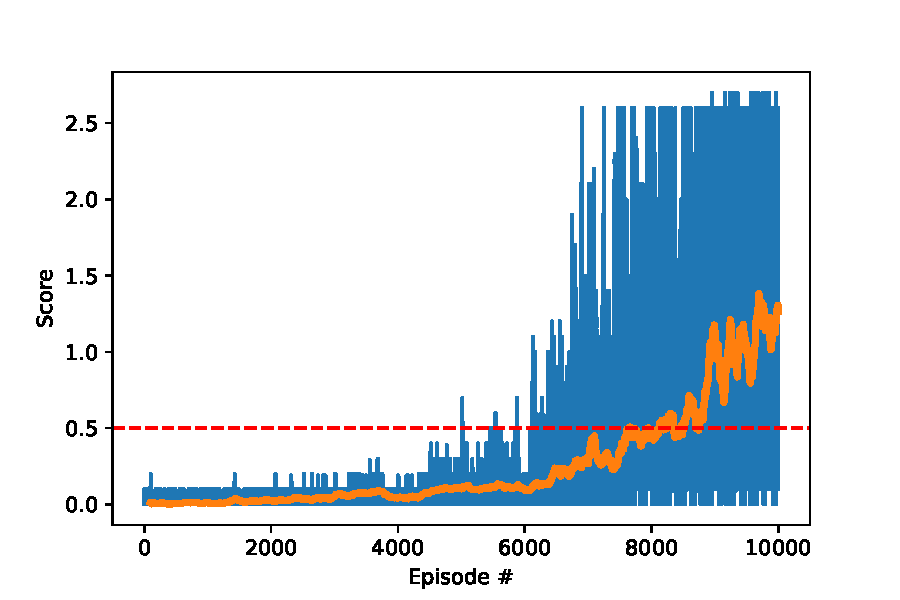
\includegraphics[page=1, height=8cm, width=14cm, angle=0]{./Plots/Average_Score.pdf}}
  \caption{Average score by episode.}
\end{figure}

%----------------------------------


%\newpage
%----------------------------------
\section{Future Work}

The current solution is quite slower than the benchmark solution, but the benchmark solutions adopts the DDPG framework which learns faster but it is seems more unstable too. 

Looking at possible ways to improve the current architecture there would be few options.

We are currently uniformly sampling from past experiences, but a prioritise sampling would likely speed up the learning.
One simple criteria would be to over weights experiences that yield a greater update.

As suggested by the MADDPG paper, one interesting route to further improve performance and stability would be to train and ensemble of policies.

\end{document}
